
%=====================================================================
\section{Polynomial symbolic complexity for finite-guard selectors}\label{sec:complexity}
%=====================================================================
Sections~\ref{sec:maxpp}--\ref{sec:freq} proved an exact complexity for one selector. This section shows that the zero entropy of its itinerary is an instance of a general mechanism: whenever the branch values are finitely many and the guards are finite arrangements of affine conditions on the valuations, the number of distinct itinerary words of length $k$ grows at most polynomially.

\subsection{The class of finite-guard selectors}
\begin{definition}[Finite-guard selector system]\label{def:finite-guard}
A \emph{finite-guard selector system} $\mathcal G$ consists of:
\begin{enumerate}[label=(\alph*),itemsep=1pt]
\item a finite set $P$ of $d$ primes; the \emph{state} is $e=(v_p(x))_{p\in P}\in\N^d$, and valuations at other primes are never read;
\item a finite set $\mathcal N$ of \emph{branch values}, $\nu=|\mathcal N|$, each $N\in\mathcal N$ being $P$-smooth, with translation vector $t_N=(2v_p(N+1)-v_p(N))_{p\in P}\in\Z^d$;
\item a finite set $Q$ of \emph{control states};
\item \emph{guard data}: real affine forms $\ell_1,\dots,\ell_r$ on $\R^d$; finite threshold sets $T_p\subset\N$ ($p\in P$) containing every $v_p(N)$, $N\in\mathcal N$, with $\tau=\sum_p|T_p|$; and a modulus $M\ge1$;
\item a rule $\Phi$ that maps the \emph{guard value}
\[
G(e)=\bigl(\operatorname{sgn}\ell_1(e),\dots,\operatorname{sgn}\ell_r(e);\ ([e_p\ge t])_{p\in P,\,t\in T_p};\ e\bmod M\bigr)
\]
and the control state $q$ to a pair $(N,q')$ with $N\in\mathcal N$ legal at $e$ (legality is read from the threshold indicators), or to a halting symbol if no branch is legal.
\end{enumerate}
The \emph{orbit} from $(e_0,q_0)$ is $e_{n+1}=e_n+t_{N_n}$, $q_{n+1}=q'_n$, with $(N_n,q'_n)=\Phi(G(e_n),q_n)$, and its \emph{branch/control itinerary} is the word $w=\bigl((N_n,q_n)\bigr)_{n\ge0}$.
\end{definition}
The functions $\Phi$ may be arbitrary; only the \emph{arguments} of $\Phi$ are restricted. Real coefficients are allowed in the forms $\ell_j$, so that conditions such as $\alpha\ln2-\beta\ln3>0$ belong to the class.

\begin{example}[Members of the class]\label{ex:members}
\begin{enumerate}[label=(\roman*),itemsep=1pt]
\item \textsf{SPF}, \textsf{LPF}, \textsf{MINPP}, \textsf{MAXPP}, started at $x_0$ and taken with $P=\{p\text{ prime}:p\le\max(3,P^+(x_0))\}$. By Corollary~\ref{cor:norenewal} the support never leaves $P$; the branch values are the primes in $P$; \textsf{SPF}/\textsf{LPF} read the indicators $[e_p\ge1]$, and \textsf{MINPP}/\textsf{MAXPP} compare $e_p\ln p$ with $e_{p'}\ln p'$, which are the signs of the affine forms $e_p\ln p-e_{p'}\ln p'$. Here $M=1$ and $|Q|=1$.
\item The tail of \textsf{MAXPP}: $P=\{2,3\}$, $\mathcal N=\{2,3\}$, one form $\ell=\alpha\ln2-\beta\ln3$, $T_2=T_3=\{0,1\}$.
\item Any rule that selects, by an arbitrary function of the divisibility pattern of $x$, among the divisors of $x$ in $[2,c]$ for a fixed $c$: $P=\{p\le c\}$, $\mathcal N=\{2,\dots,c\}$, and the thresholds $v_p(d)$, $d\le c$. Primes larger than $c$ may appear in the integer but are never read.
\item Rules with a finite memory (a finite control $Q$) and rules that read residues of the valuations modulo $M$.
\end{enumerate}
\end{example}

\subsection{Counting faces of an arrangement}
\begin{lemma}[Regions of an arrangement]\label{lem:regions}
Let $H_1,\dots,H_n$ be affine hyperplanes in $\R^d$. The complement $\R^d\setminus\bigcup H_i$ has at most $\sum_{i=0}^{d}\binom ni$ connected components.
\end{lemma}
\begin{lemma}[Faces of an arrangement]\label{lem:faces}
Let $g_1,\dots,g_n$ ($n\ge1$) be affine functions on $\R^d$. The number of distinct sign vectors $(\operatorname{sgn}g_1(y),\dots,\operatorname{sgn}g_n(y))\in\{-,0,+\}^n$, $y\in\R^d$, is at most $c_dn^d$ with $c_d=\frac{(d+1)(d+2)}2$.
\end{lemma}
Both lemmas are classical (Buck, Zaslavsky); complete short proofs are in Appendix~\ref{app:classical}.

\begin{theorem}[Polynomial complexity for finite-guard selectors]\label{thm:E}
Let $\mathcal G$ be a finite-guard selector system with parameters $d,\nu=|\mathcal N|,|Q|,M,r,\tau$ as in Definition~\ref{def:finite-guard}. Let $W_k$ be the set of all words of length $k$ (words that stop at a halting symbol being counted too) that occur as the first $k$ letters of the branch/control itinerary of some orbit, over \emph{all} initial states $(e_0,q_0)\in\N^d\times Q$. Then
\[
|W_k|\ \le\ |Q|\,M^d\,c_d\,n_k^d,\qquad n_k=(r+\tau)\,|S_k|,\qquad |S_k|\le\binom{k-1+\nu}{\nu}\le k^\nu,
\]
so $|W_k|\le |Q|M^dc_d(r+\tau)^d\,k^{d\nu}$ is polynomial in $k$. Consequently every orbit has a branch/control itinerary of topological entropy $0$, and so does every finite coding of it (any map from the finite alphabet $\mathcal N\times Q$ applied letter by letter, or through a sliding block of fixed width).
\end{theorem}
\noindent\emph{Source.} Theorem GEN-C3 of U4-GEN-C~\cite{u4genc} (not part of the collection~\cite{coll}) concerns selectors with finitely many branch values and log-linear, threshold and congruence guards. The hypotheses of the theorem above are the finite-guard hypotheses of Definition~\ref{def:finite-guard}; finiteness of the branch set alone is not sufficient for polynomial complexity. The quantitative corollary GEN-C3a of that release was withdrawn in U4-GEN-C-ORDER~\cite{u4order} (ORD-0, E1) and is not used here; the bound is the one proved in this section.
\begin{proof}
Let $S_k\subset\Z^d$ be the set of sums of at most $k-1$ vectors $t_N$, $N\in\mathcal N$. The sums of exactly $j$ vectors correspond to multisets of size $j$ in $\mathcal N$, so $|S_k|\le\sum_{j\le k-1}\binom{j+\nu-1}{\nu-1}=\binom{k-1+\nu}\nu$, and $\binom{k-1+\nu}{\nu}=\prod_{i=1}^{\nu}\frac{k-1+i}{i}\le k^\nu$. 
Consider the family $\mathcal F_k$ of affine functions on $\R^d$
\[
e\mapsto\ell_j(e+s)\ (1\le j\le r),\qquad e\mapsto e_p+s_p-t\ (p\in P,\ t\in T_p),\qquad s\in S_k;
\]
it has $n_k'\le n_k$ members. For $e\in\N^d$ let $\sigma(e)$ be its sign vector under $\mathcal F_k$ (its \emph{face}).

\emph{Claim.} If $e_0,e_0'\in\N^d$ satisfy $\sigma(e_0)=\sigma(e_0')$ and $e_0\equiv e_0'\pmod M$, and $q_0=q_0'$, then the first $k$ letters (and the halting behaviour) of the two itineraries coincide.

Proof of the claim by induction on the step $i<k$: suppose the letters up to step $i-1$ coincide, hence the control states $q_i=q_i'$ and the accumulated displacement $s_i=\sum_{m<i}t_{N_m}\in S_k$ coincide, and $e_i=e_0+s_i$, $e_i'=e_0'+s_i$. Then $\operatorname{sgn}\ell_j(e_i)=\operatorname{sgn}\ell_j(e_i')$ and $[ (e_i)_p\ge t]=[(e_i')_p\ge t]$ because these are members of $\sigma(e_0)=\sigma(e_0')$ with $s=s_i$; and $e_i\equiv e_i'\pmod M$. Hence $G(e_i)=G(e_i')$, $\Phi$ gives the same pair $(N_i,q_{i+1})$, and the same halting decision.

By the claim a word in $W_k$ is determined by the triple $(\sigma(e_0),\,e_0\bmod M,\,q_0)$. By Lemma~\ref{lem:faces} there are at most $c_dn_k^d$ faces, there are $M^d$ residues and $|Q|$ control states. This gives the bound. 
For a coded sequence, a block of length $k$ of the coded sequence is the image of a block of length $k+s$ ($s$ the block width minus one) of the original; hence the coded complexity is at most $|W_{k+s}|$, which is polynomial, and the entropy is $\lim\frac1k\ln|W_{k+s}|=0$. Every factor of length $k$ of an itinerary is the initial word of the orbit started at a later state, hence lies in $W_k$; so $p(k)\le|W_k|$ and the entropy is $0$ by Lemma~\ref{lem:entropy}. \end{proof}

\begin{corollary}[Positive entropy needs more than finitely many affine branches]\label{cor:needs}
If a selector has finitely many branch values and finite-guard type, its branch/control itinerary has entropy $0$. Hence a selector whose branch/control itinerary has positive entropy has infinitely many branch values or guards that are not of finite-guard type.
\end{corollary}
Finite branch sets imply finite total prime support (Theorem~\ref{thm:D}); the finite-guard hypotheses of Definition~\ref{def:finite-guard} are an additional restriction on how the selector decides, and under them Theorem~\ref{thm:E} gives polynomial complexity. \textsf{MAXPP} attains the smallest unbounded value, $p(k)=k+1$.

\begin{remark}[Scope]\label{rem:scope}
Theorem~\ref{thm:E} is a statement about finite codings of the \emph{branch/control itinerary}. It does not assert zero entropy for arbitrary finite-valued observations of the full integer state $x_n$, nor for observations of a branch itinerary with infinitely many values; Section~\ref{sec:order} shows that observations of the latter kind can have positive entropy.
\end{remark}

\subsection{Computed instances}
Theorem~\ref{thm:E} was tested on thirty random finite-guard systems with $d\in\{2,3\}$, $2$--$4$ branch values, up to three affine forms with real coefficients, thresholds, moduli $M\le3$, up to three control states and pseudo-random rules $\Phi$ (the rule is a hash table of the guard value, so it has no structure beyond the arguments): (a) $16\,839$ pairs of starts with equal faces and equal residues produced equal words of length $6$ with no exception; (b) for each system and each $k=2,\dots,6$ the exhaustive number of words obtained from all starts in a box and all control states is below the bound of the theorem. Table~\ref{tab:thmE} lists eight of the thirty systems.
\begin{table}[ht]\centering\small
\begin{tabular}{@{}rrrrrr@{}}\toprule
$d$ & $|\mathcal N|$ & $|Q|$ & $M$ & $p_{\rm all}(6)$ & bound of Thm~\ref{thm:E}\\\midrule
3 & 2 & 1 & 1 & 37 & 47\,416\,320 \\
2 & 3 & 2 & 3 & 182 & 21\,676\,032 \\
2 & 2 & 1 & 2 & 54 & 381\,024 \\
3 & 2 & 2 & 3 & 1422 & 6\,656\,251\,140 \\
2 & 3 & 3 & 1 & 66 & 3\,612\,672 \\
2 & 3 & 3 & 3 & 756 & 50\,803\,200 \\
3 & 4 & 3 & 2 & 1466 & 480\,090\,240\,000 \\
3 & 4 & 3 & 2 & 1923 & 639\,000\,109\,440 \\
\bottomrule\end{tabular}

\caption{Computed words of length $6$ over all starts in a box versus the bound of Theorem~\ref{thm:E} (first eight of thirty systems; $d$ primes, $\nu$ branches, $|Q|$ control states, modulus $M$).}\label{tab:thmE}\end{table}

%=====================================================================
\section{Exponent-profile observables and arithmetic counters}\label{sec:order}
%=====================================================================
Theorem~\ref{thm:E} excluded infinitely many branch values. This section treats the simplest selector that has them, a counter, and shows what a finite-valued observable of its itinerary can look like.

\subsection{A state-only counter}
Fix $m_0\ge2$ and put, for $m\ge m_0$,
\[
D(m)=\frac{m\cdot m!}{m_0!},\qquad S(x)=\max\{m\ge m_0:\ D(m)\mid x\}\quad(\text{for }m_0\mid x),
\]
and let $S(x)$ be any legal branch (say the smallest prime factor) if $m_0\nmid x$.
\begin{theorem}[Counter selector]\label{thm:ordS}
The selector $S$ is autonomous (a function of the current integer alone), and the orbit from $x_0=m_0$ is
\[
x_j=\frac{(m_0+j)\,(m_0+j)!}{m_0!},\qquad N_j=S(x_j)=m_0+j\qquad(j\ge0).
\]
\end{theorem}
\noindent\emph{Source.} The counter selector is the decoder construction of U4-GEN-C-ORDER~\cite{u4order} (ORD-3), a release that is not part of the collection~\cite{coll}.
\begin{proof}
Put $m=m_0+j$. Then $D(m)=x_j$, and $D(m)\mid x_j$. Since $D(m+1)/D(m)=(m+1)^2/m>1$, $D$ is strictly increasing, so $D(m')>x_j$ and $D(m')\nmid x_j$ for $m'>m$. Hence $S(x_j)=m$. The branch $N_j=m$ is legal because $m\mid m\cdot m!/m_0!=x_j$ (the quotient $m!/m_0!$ is an integer). Finally $T_m(x_j)=x_j\frac{(m+1)^2}m=\frac{m!\,(m+1)^2}{m_0!}=\frac{(m+1)(m+1)!}{m_0!}=x_{j+1}$. For $j=0$, $x_0=m_0\cdot m_0!/m_0!=m_0$. \end{proof}
The itinerary is injective, $N_{j+1}=N_j+1$: the selector implements a counter, with unboundedly many branch values. By Theorem~\ref{thm:D} its prime support renews, as it must.

\subsection{The exponent-profile observable}
For $m\ge1$ let $E(m)=\{v_p(m):p\mid m\}$ be the set of its prime exponents and define
\[
u(m)=\begin{cases}0,&|E(m)|\le1\ (\text{all exponents equal, or }m=1),\\ 1,&\text{otherwise.}\end{cases}
\]
\begin{lemma}\label{lem:u}
$u(m)=0$ iff $m=s^e$ for a squarefree $s$ and an integer $e\ge1$ (or $m=1$).
\end{lemma}
\begin{proof} If all exponents equal $e$, then $m=\prod p^e=(\prod p)^e$; the converse is clear. \end{proof}
The observable of the counter itinerary is the $\{0,1\}$-valued sequence $o_j=u(N_j)=u(m_0+j)$. Along the orbit it can also be read from the state: $o(x)=u(S(x))$. Its early values and block counts are shown in Figure~\ref{fig:order} and Table~\ref{tab:orderblocks}.

\begin{theorem}[Positive entropy of the exponent-profile observable]\label{thm:ordE}
For every $k\ge1$ the sequence $(u(m))_{m\ge m_0}$ contains at least $2^{\lceil 2k/\pi^2\rceil}$ distinct words of length $k$, each of which occurs infinitely often. Consequently its topological entropy is at least $\frac2{\pi^2}\ln2\approx0.1405$ nats per letter.
\end{theorem}
\noindent\emph{Source.} This is Theorem ORD-E, with Corollary ORD-C for the selector $S$, of U4-GEN-C-ORDER~\cite{u4order}. The proof given here is self-contained.
\begin{proof}
Fix $k\ge2$ (for $k=1$ both values occur infinitely often: $u(p)=0$ for primes $p$ and $u(4p)=1$ for odd primes $p$). Let $\mathcal L$ be the set of odd primes $\le k$, and
\[
Q_0=4\prod_{l\in\mathcal L}l^2 .
\]
\emph{Step 1: good positions.} For a residue $r\bmod Q_0$ put
\[
E_r=\{\,i\in[1,k]:\ r+i\equiv2\!\!\pmod4\ \text{ and }\ l^2\nmid r+i\ \text{ for all }l\in\mathcal L\,\}.
\]
Membership depends only on $r\bmod Q_0$. As $r$ runs over $\Z/Q_0\Z$, $r+i$ runs uniformly, and by the Chinese remainder theorem the conditions modulo $4$ and modulo the $l^2$ are independent with probabilities $\frac14$ and $1-l^{-2}$. Hence
\[
\frac1{Q_0}\sum_{r}|E_r|=k\,d_k,\qquad d_k=\frac14\prod_{l\in\mathcal L}\Bigl(1-\frac1{l^2}\Bigr)\ \ge\ \frac14\prod_{l\ \text{odd prime}}\Bigl(1-\frac1{l^2}\Bigr)=\frac14\cdot\frac{6/\pi^2}{1-1/4}=\frac2{\pi^2},
\]
using Euler's product $\prod_{l}(1-l^{-2})=1/\zeta(2)=6/\pi^2$ over all primes. Choose $r$ with $|E_r|\ge kd_k$; as $|E_r|$ is an integer, $|E_r|\ge\lceil2k/\pi^2\rceil=:\kappa$. Fix such an $r$ and a set $E\subset E_r$ with $|E|=\kappa$.

\emph{Step 2: prescribing patterns.} Let $\varepsilon\in\{0,1\}^E$. Let $E_1=\{i:\varepsilon_i=1\}$, $E_0=E\setminus E_1$, and choose distinct primes $p_i>k$ ($i\in E_1$); they do not divide $Q_0$. By the Chinese remainder theorem the system
\[
m\equiv r\ (\mathrm{mod}\ Q_0),\qquad m\equiv-i\ (\mathrm{mod}\ p_i^2)\ (i\in E_1)
\]
is a residue class $m\equiv m^*\pmod Q$ with $Q=Q_0\prod_{i\in E_1}p_i^2$. For $m$ in this class and $i\in E$ put $n=m+i$. Then $v_2(n)=1$ and $v_l(n)\le1$ for all $l\in\mathcal L$. Therefore:
\begin{itemize}[itemsep=1pt]
\item if $i\in E_1$, then $p_i^2\mid n$, so the exponent of $p_i$ differs from the exponent $1$ of $2$ and $u(n)=1$;
\item if $i\in E_0$ and no prime $q>k$ satisfies $q^2\mid n$, then every prime exponent of $n$ equals $1$ and $u(n)=0$.
\end{itemize}
It remains to find $m$ in the class for which, for every $i\in E_0$, no prime $q>k$ has $q^2\mid m+i$. For $q=p_j$ ($j\in E_1$) this holds automatically: $p_j^2\mid m+j$, so $p_j^2\mid m+i$ would give $p_j^2\mid i-j$, but $0<|i-j|<k<p_j^2$.

\emph{Step 3: a density argument.} Take $m=m^*+Qt$, $0\le t<T$. For a prime $q>k$ not among the $p_j$, $\gcd(q^2,Q)=1$, so $q^2\mid m^*+i+Qt$ for at most $T/q^2+1$ values of $t$, and only for $q^2\le QT+k$. The number of ``bad'' $t$ is at most
\[
\sum_{i\in E_0}\ \sum_{\substack{q>k\\ q^2\le QT+k}}\Bigl(\frac T{q^2}+1\Bigr)\ \le\ kT\sum_{q>k}\frac1{q^2}+k\sqrt{QT+k}.
\]
Primes $q>k\ge2$ are odd, and for odd $n\ge n_0$ one has $\frac1{n^2}<\frac1{n^2-1}=\frac12\bigl(\frac1{n-1}-\frac1{n+1}\bigr)$, which telescopes over odd $n$ to $\sum_{n\ge n_0,\,n\text{ odd}}n^{-2}<\frac1{2(n_0-1)}$. With $n_0\ge k+1$ we get $\sum_{q>k}q^{-2}<\frac1{2k}$, so the number of bad $t$ is below $\frac T2+k\sqrt{QT+k}$. Since $k$ and $Q$ are fixed, for $T$ large this is below $2T/3$, so more than $T/3$ values of $t$ are good; letting $T\to\infty$ shows that infinitely many good $m$ exist. For each of them, $u(m+i)=\varepsilon_i$ for all $i\in E$.

\emph{Conclusion.} For each of the $2^\kappa$ patterns $\varepsilon$ the word $u(m+1)\cdots u(m+k)$ at a good $m$ has $\varepsilon$ on the coordinate set $E$; distinct patterns give distinct words, each occurring infinitely often (and in particular at some $m\ge m_0$). Thus there are at least $2^{\lceil2k/\pi^2\rceil}$ words of length $k$, and $h\ge\lim\frac1k\ln2^{\lceil2k/\pi^2\rceil}=\frac2{\pi^2}\ln2$. \end{proof}

\begin{table}[ht]\centering\small
\begin{tabular}{@{}rrrr@{}}\toprule
$k$ & $p_u(k)$ (computed) & $2^k$ & $2^{\lceil 2k/\pi^2\rceil}$ (proved lower bound)\\\midrule
1 & 2 & 2 & 2 \\
2 & 4 & 4 & 2 \\
3 & 8 & 8 & 2 \\
4 & 16 & 16 & 2 \\
5 & 32 & 32 & 4 \\
6 & 64 & 64 & 4 \\
7 & 128 & 128 & 4 \\
8 & 255 & 256 & 4 \\
9 & 500 & 512 & 4 \\
10 & 935 & 1024 & 8 \\
11 & 1628 & 2048 & 8 \\
12 & 2602 & 4096 & 8 \\
13 & 4105 & 8192 & 8 \\
14 & 6262 & 16384 & 8 \\
\bottomrule\end{tabular}

\caption{Block counts $p_u(k)$ of $u$ along the integers $2\le m\le 3\cdot10^7$ (computed) against $2^{\lceil 2k/\pi^2\rceil}$ (proved lower bound); the density of $u=1$ in this range is $0.3920$.}\label{tab:orderblocks}\end{table}
\begin{table}[ht]\centering\small
\begin{tabular}{@{}rrrr@{}}\toprule
$k$ & $|E_r|$ & patterns $2^{|E_r|}$ & realised by an explicit $m$\\\midrule
10 & 3 & 8 & 8 \\
14 & 4 & 16 & 16 \\
18 & 5 & 32 & 32 \\
\bottomrule\end{tabular}

\caption{The construction of Theorem~\ref{thm:ordE} carried out explicitly (computed): for window length $k$, the number $|E|$ of controlled positions, the number $2^{|E|}$ of prescribed patterns and the number realised by explicit integers $m$ found from the Chinese-remainder system.}\label{tab:ordercrt}\end{table}
\begin{figure}[ht]\centering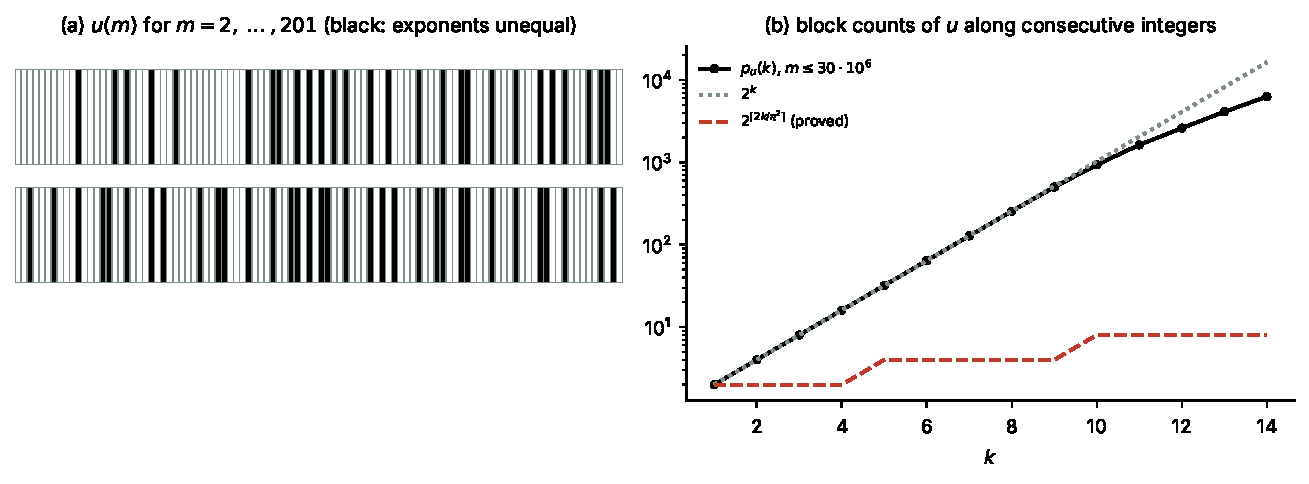
\includegraphics[width=.98\textwidth]{../figures/fig8_order.pdf}
\caption{(a) The observable $u(m)$ for $2\le m\le201$. (b) Block counts of $u$ against the proved bound; the computed counts equal $2^k$ for $k\le7$.}\label{fig:order}\end{figure}

\subsection{Generated complexity versus revealed complexity}
Two different things can be called the symbolic complexity of a selector, and the counter separates them.

\emph{Generated selection complexity} is the complexity of the itinerary produced by the selection dynamics: for \textsf{MAXPP}, a Sturmian word with $p(k)=k+1$ produced by an irrational rotation with two branch values; for the counter, the injective word $N_j=m_0+j$ produced by the translation $j\mapsto j+1$. Neither is chaotic in any sense; the mechanism of the counter is addition of one.

\emph{Arithmetic complexity revealed by an observable} is the complexity of a finite-valued function of the branch value. For the counter it is a statement about the multiplicative structure of consecutive integers: the exponent profile of $m$, $m+1,\dots$ is as free as the Chinese remainder theorem permits, and the entropy $\ge\frac{2}{\pi^2}\ln 2$ is a property of the integer sequence $(u(m))_{m\ge m_0}$, not of the selector that enumerates it.

Consequently a positive entropy of a fixed finite observable of a branch itinerary with unboundedly many values must not be read as chaos of the selection dynamics; the dynamics here is a counter. Conversely, Theorem~\ref{thm:E} shows that for finitely many branches and finite-guard decisions no finite coding of the branch/control itinerary has positive entropy, and Theorem~\ref{thm:B} shows what the dynamics actually generates in the \textsf{MAXPP} case.

\begin{proposition}[A self-referential selector]\label{prop:ord2}
Let $N_n=x_n$, i.e.\ $x_{n+1}=(x_n+1)^2$. For $n\ge2$ one has $x_n\equiv1\pmod3$; the parity of $x_n$ alternates; every odd iterate with $n\ge1$ is $\equiv1\pmod8$ and every even iterate with $n\ge2$ has $v_2(x_n)=2$. Moreover, for any finite set of primes $P$ and cap $c$, the vector $(\min(v_p(x_n),c))_{p\in P}$ is a function of $x_n\bmod\prod_{p\in P}p^c$ and is eventually periodic in $n$.
\end{proposition}
\noindent\emph{Source.} Lemma ORD-2b of U4-GEN-C-ORDER~\cite{u4order} gives the periodicity statement.
\begin{proof}
$x\mapsto(x+1)^2$ preserves congruence classes: $x\equiv0,1\bmod3$ gives $(x+1)^2\equiv1$ and $x\equiv2$ gives $0$, after which the next iterate is $\equiv1$; so $x_n\equiv1\ (3)$ for $n\ge2$. If $x$ is even then $(x+1)^2$ is an odd square, hence $\equiv1\pmod8$; if $x$ is odd then $x+1$ is even and $(x+1)^2$ is even, so the parity alternates. For an even $x_n$ with $n\ge2$ the predecessor $x_{n-1}$ is odd and, being $(x_{n-2}+1)^2$ with $x_{n-2}$ even, is an odd square, hence $\equiv1\pmod8$; so $x_{n-1}+1\equiv2\pmod8$ and $v_2(x_n)=2v_2(x_{n-1}+1)=2$. Finally $x_{n+1}\bmod M$ depends only on $x_n\bmod M$ with $M=\prod_{p\in P}p^c$, a finite set of residues, so the residue orbit is eventually periodic and so is the capped valuation vector. \end{proof}
\begin{remark}
The proposition shows that a state-reading selector with $N=x$ keeps all bounded-profile observables eventually periodic: the unbounded exponents of the counter in Theorem~\ref{thm:ordE} are what carries the entropy there. (Verified in checks C11c, C11g for starts $4\le x_0<1700$.)
\end{remark}
